\documentclass[aspectratio=169]{beamer}
\usetheme{Madrid}
\usecolortheme{dolphin}
\usepackage[utf8]{inputenc}
\usepackage[T1]{fontenc}
\usepackage[english]{babel}
\usepackage{lmodern}
\usepackage{hyperref}
\usepackage{booktabs}
\usepackage{tikz}
\usepackage{xcolor}
\usepackage{colortbl}

\title{AI for Theory}
\subtitle{State of the art, uses and actions for the community}
\author{Gabriel Peyré \\ CNRS and ENS, Université PSL}
\date{July 2, 2026}

\definecolor{aiNavy}{HTML}{26364F}
\definecolor{aiBlue}{HTML}{2F6FA3}
\definecolor{aiTeal}{HTML}{238C82}
\definecolor{aiGreen}{HTML}{3F8A5F}
\definecolor{aiAmber}{HTML}{B7791F}
\definecolor{aiRed}{HTML}{A84E4E}
\definecolor{aiViolet}{HTML}{6C63C7}
\definecolor{aiSlate}{HTML}{6D7480}
\definecolor{softBlue}{HTML}{EAF2FB}
\definecolor{softTeal}{HTML}{E6F5F2}
\definecolor{softGreen}{HTML}{ECF7EE}
\definecolor{softAmber}{HTML}{FFF2D7}
\definecolor{softRed}{HTML}{FBEDED}
\definecolor{softViolet}{HTML}{F0EEFB}
\definecolor{softGray}{HTML}{F4F6F8}
\definecolor{softGrayA}{HTML}{F7F8FA}
\definecolor{softGrayB}{HTML}{F1F4F7}
\definecolor{softGrayC}{HTML}{ECEFF3}
\definecolor{softGrayD}{HTML}{F5F5F2}
\definecolor{softGrayE}{HTML}{F0F2F4}

\setbeamercolor{structure}{fg=aiBlue}
\setbeamercolor{title}{fg=aiNavy}
\setbeamercolor{subtitle}{fg=aiBlue}
\setbeamercolor{frametitle}{fg=aiNavy,bg=softBlue}
\setbeamerfont{frametitle}{series=\bfseries}
\setbeamercolor{palette primary}{fg=white,bg=aiNavy}
\setbeamercolor{palette secondary}{fg=white,bg=aiBlue}
\setbeamercolor{palette tertiary}{fg=white,bg=aiTeal}
\setbeamercolor{palette quaternary}{fg=white,bg=aiViolet}
\setbeamercolor{box claim}{fg=black,bg=softGrayA}
\setbeamercolor{box proof}{fg=black,bg=softGrayB}
\setbeamercolor{box example}{fg=black,bg=softGrayC}
\setbeamercolor{box action}{fg=black,bg=softGrayD}
\setbeamercolor{box risk}{fg=black,bg=softGrayE}
\setbeamercolor{box danger}{fg=black,bg=softGrayC}
\setbeamercolor{box neutral}{fg=black,bg=softGrayA}
\setbeamercolor{box neutral alt}{fg=black,bg=softGrayC}
\setbeamercolor{box problem}{fg=black,bg=softBlue}
\setbeamercolor{box result}{fg=black,bg=softTeal}
\setbeamercolor{box takeaway}{fg=black,bg=softAmber}
\setbeamertemplate{itemize item}{\raise0.15ex\hbox{\scriptsize\color{aiBlue}\(\blacktriangleright\)}}
\setbeamertemplate{itemize subitem}{\raise0.15ex\hbox{\tiny\color{aiTeal}\(\blacktriangleright\)}}
\setbeamertemplate{blocks}[rounded][shadow=false]

\newcommand{\source}[1]{\vspace{1mm}{\tiny\color{aiSlate}Source: #1}}
\newenvironment{claimbox}{\begin{beamercolorbox}[wd=\linewidth,rounded=true,sep=1.1mm]{box claim}}{\end{beamercolorbox}}
\newenvironment{proofbox}{\begin{beamercolorbox}[wd=\linewidth,rounded=true,sep=1.1mm]{box proof}}{\end{beamercolorbox}}
\newenvironment{examplebox}{\begin{beamercolorbox}[wd=\linewidth,rounded=true,sep=1.1mm]{box example}}{\end{beamercolorbox}}
\newenvironment{actionbox}{\begin{beamercolorbox}[wd=\linewidth,rounded=true,sep=1.1mm]{box action}}{\end{beamercolorbox}}
\newenvironment{riskbox}{\begin{beamercolorbox}[wd=\linewidth,rounded=true,sep=1.1mm]{box risk}}{\end{beamercolorbox}}
\newenvironment{dangerbox}{\begin{beamercolorbox}[wd=\linewidth,rounded=true,sep=1.1mm]{box danger}}{\end{beamercolorbox}}
\newenvironment{neutralbox}{\begin{beamercolorbox}[wd=\linewidth,rounded=true,sep=1.1mm]{box neutral}}{\end{beamercolorbox}}
\newenvironment{neutralboxalt}{\begin{beamercolorbox}[wd=\linewidth,rounded=true,sep=1.1mm]{box neutral alt}}{\end{beamercolorbox}}
\newenvironment{problembox}{\begin{beamercolorbox}[wd=\linewidth,rounded=true,sep=1.0mm]{box problem}}{\end{beamercolorbox}}
\newenvironment{resultbox}{\begin{beamercolorbox}[wd=\linewidth,rounded=true,sep=1.0mm]{box result}}{\end{beamercolorbox}}
\newenvironment{takeawaybox}{\begin{beamercolorbox}[wd=\linewidth,rounded=true,sep=1.0mm]{box takeaway}}{\end{beamercolorbox}}
\newcommand{\problemlabel}{\textbf{\textcolor{aiBlue}{Problem}}}
\newcommand{\resultlabel}{\textbf{\textcolor{aiTeal}{Results}}}
\newcommand{\takeawaylabel}{\textbf{\textcolor{aiAmber}{Takeaway}}}
\newlength{\keylabelwidth}
\newcommand{\keyitem}[2]{%
  \item \settowidth{\keylabelwidth}{\textbf{#1}: }%
  \makebox[\keylabelwidth][l]{\textbf{#1}: }%
  \parbox[t]{\dimexpr\linewidth-\keylabelwidth-0.6em\relax}{\raggedright #2}%
}
\newcommand{\keyline}[2]{%
  \settowidth{\keylabelwidth}{\textbf{#1}: }%
  \noindent\makebox[\keylabelwidth][l]{\textbf{#1}: }%
  \parbox[t]{\dimexpr\linewidth-\keylabelwidth-0.6em\relax}{\raggedright #2}\par%
}
\newcommand{\labelline}[2]{%
  \settowidth{\keylabelwidth}{#1 : }%
  \noindent\makebox[\keylabelwidth][l]{#1 : }%
  \parbox[t]{\dimexpr\linewidth-\keylabelwidth-0.6em\relax}{\raggedright #2}\par%
}
\newcommand{\plantile}[7]{%
  \begin{scope}[shift={(#1,#2)},opacity=#7]
    \filldraw[fill=#5,draw=aiSlate!38,line width=0.65pt,rounded corners=2.5pt] (0,0) rectangle (5.72,2.62);
    \draw[#6!60,line width=1.0pt] (0.20,0.28) -- (0.20,2.36);
    \node[anchor=north west,font=\bfseries\large,text=black,inner sep=0pt,align=left,text width=5.15cm] at (0.38,2.38) {#3};
    \begin{scope}
      \clip[rounded corners=1.5pt] (0.30,0.24) rectangle (5.42,1.56);
      \node[inner sep=0pt] at (2.86,0.90) {\includegraphics[width=5.12cm,height=1.32cm,keepaspectratio]{#4}};
    \end{scope}
  \end{scope}
}
\newcommand{\planslide}[1]{%
\ifnum#1=1\def\planopone{1}\else\def\planopone{0.34}\fi
\ifnum#1=2\def\planoptwo{1}\else\def\planoptwo{0.34}\fi
\ifnum#1=3\def\planopthree{1}\else\def\planopthree{0.34}\fi
\ifnum#1=4\def\planopfour{1}\else\def\planopfour{0.34}\fi
\begin{frame}{Talk roadmap}
\vspace{-1mm}
\begin{center}
\begin{tikzpicture}[x=1cm,y=1cm]
  \plantile{0}{3.02}{LLMs and mathematics}{assets/generated/imo_2025_problem1_crop.png}{softGrayA}{aiBlue}{\planopone}
  \plantile{6.02}{3.02}{AI for research\\in mathematics}{assets/generated/unit_distance_series.png}{softGrayB}{aiTeal}{\planoptwo}
  \plantile{0}{0.12}{Experience reports}{assets/generated/noogram_flow_matching_site.png}{softGrayD}{aiAmber}{\planopthree}
  \plantile{6.02}{0.12}{Impact on the\\community}{assets/generated/paperreview_ai_screenshot.png}{softGrayC}{aiViolet}{\planopfour}
\end{tikzpicture}
\end{center}
\end{frame}
}

\begin{document}

\begin{frame}[plain]
\centering
\vspace{1.25cm}
{\fontsize{34}{40}\selectfont\bfseries\textcolor{aiNavy}{AI for Theory}\par}
\vspace{0.45cm}
{\Large\textcolor{aiBlue}{State of the art, uses and actions for the community}\par}
\vspace{0.9cm}
{\large Gabriel Peyré\par}
\vspace{0.15cm}
{\normalsize\textcolor{aiSlate}{CNRS and ENS, Université PSL}\par}
\vfill
{\small\textcolor{aiSlate}{July 2, 2026}\par}
\vspace{0.18cm}
{\scriptsize\href{https://github.com/gpeyre/ia4maths}{\textcolor{aiBlue}{\texttt{github.com/gpeyre/ia4maths}}}\par}
\end{frame}

\planslide{1}

\begin{frame}{AI for mathematics}
\small
\begin{columns}[T,totalwidth=\linewidth]
\column{0.49\linewidth}
\begin{actionbox}
\textbf{AI for scientific discovery}\par
\vspace{1mm}
{\centering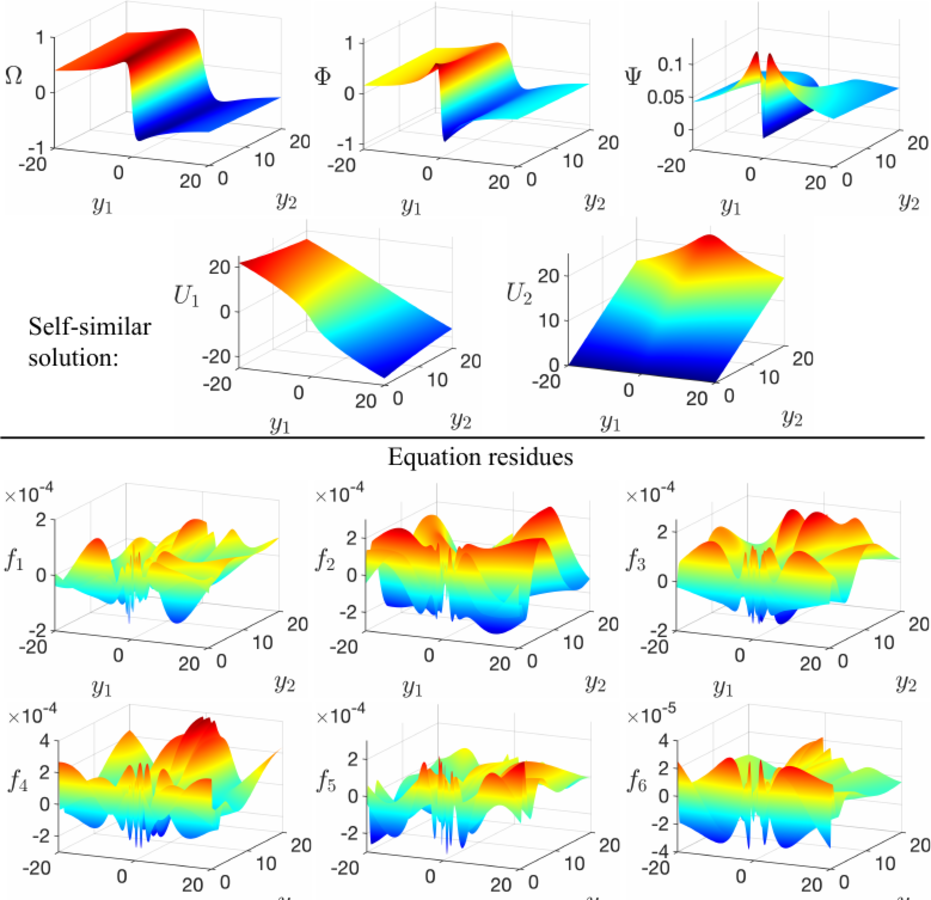
\includegraphics[height=0.34\textheight,keepaspectratio]{assets/generated/euler_pinn_blowup_crop.png}\par}
\vspace{0.5mm}
\raggedright{\scriptsize PINNs to explore PDEs: Navier--Stokes / Euler, instabilities, counterexamples.}
\end{actionbox}

\column{0.49\linewidth}
\begin{proofbox}
\textbf{AI for theorem proving}\par
\vspace{1mm}
{\centering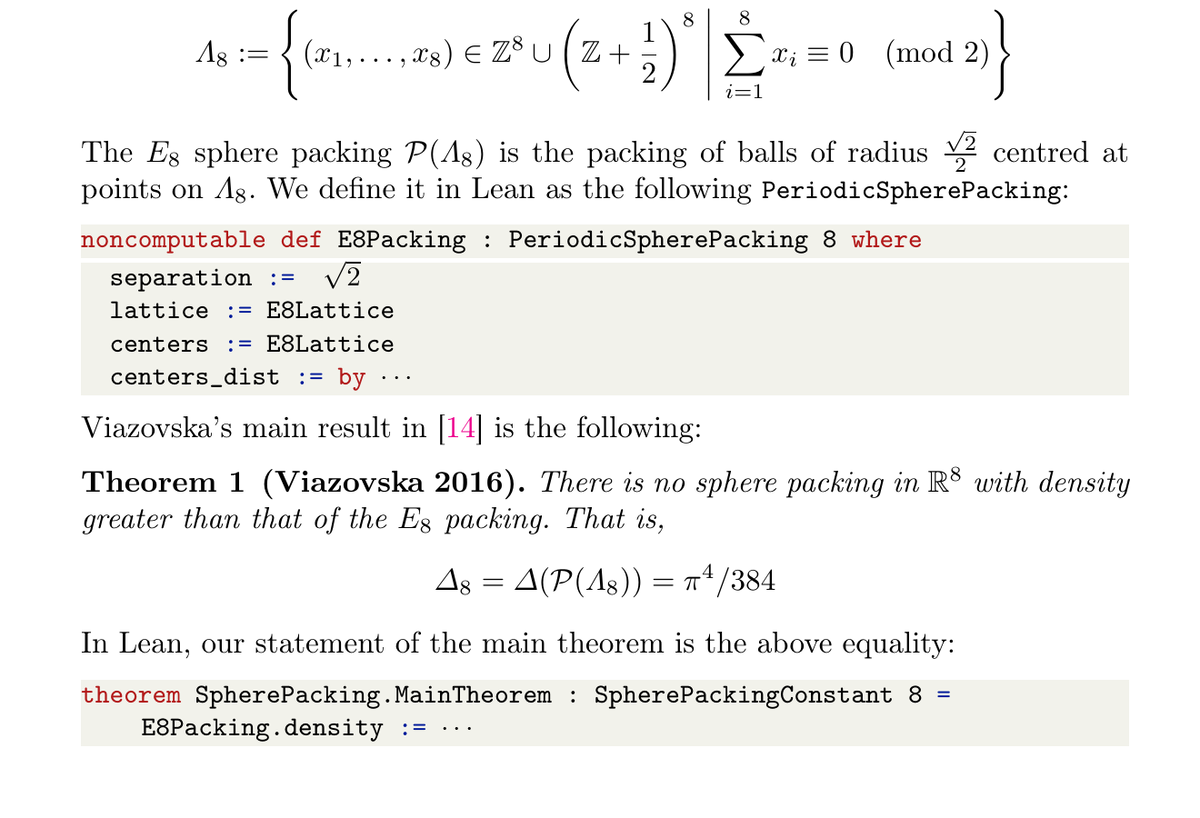
\includegraphics[height=0.32\textheight,keepaspectratio]{assets/generated/sphere_packing_lean_crop.png}\par}
\vspace{0.5mm}
\raggedright{\scriptsize Lean: verified proof; Viazovska's optimal \(E_8\) packing.}
\end{proofbox}
\end{columns}

\vspace{1mm}
\begin{claimbox}
\textbf{Focus}: mathematical reasoning, from informal to formal.
\end{claimbox}
\source{Wang--Lai--Gómez-Serrano--Buckmaster, arXiv:2201.06780 ; Hariharan et al., arXiv:2604.23468.}
\end{frame}

\begin{frame}{LLMs for reasoning and mathematics}
\small
\begin{center}
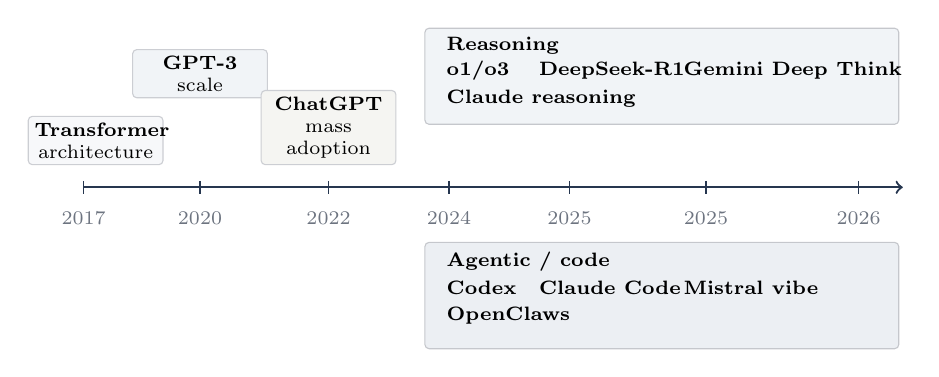
\begin{tikzpicture}[x=1.02cm,y=1cm]
  \tikzset{
    foundation/.style={font=\scriptsize,align=center,text width=1.55cm,inner sep=2.3pt,draw=aiSlate!35,fill=softGrayA,rounded corners=1.5pt},
    tag/.style={font=\scriptsize,anchor=west}
  }
  \draw[->,thick,aiNavy] (0,0) -- (10.2,0);
  \foreach \x/\y in {0/2017,1.45/2020,3.05/2022,4.55/2024,6.05/2025,7.75/2025,9.65/2026}
    {\draw[aiNavy] (\x,0.08) -- (\x,-0.08) node[below=3pt,text=aiSlate] {\scriptsize \y};}

  \node[foundation,anchor=south] at (0.15,0.28)
    {\textbf{Transformer}\\architecture};
  \node[foundation,fill=softGrayB,anchor=south] at (1.45,1.13)
    {\textbf{GPT-3}\\scale};
  \node[foundation,fill=softGrayD,anchor=south] at (3.05,0.28)
    {\textbf{ChatGPT}\\mass adoption};

  \filldraw[draw=aiSlate!40,fill=softGrayB,rounded corners=1.5pt] (4.25,0.80) rectangle (10.15,2.02);
  \node[tag] at (4.40,1.80) {\textbf{Reasoning}};
  \node[tag] at (4.40,1.48) {\textbf{o1/o3}};
  \node[tag] at (5.55,1.48) {\textbf{DeepSeek-R1}};
  \node[tag] at (7.35,1.48) {\textbf{Gemini Deep Think}};
  \node[tag] at (4.40,1.12) {\textbf{Claude reasoning}};

  \filldraw[draw=aiSlate!40,fill=softGrayC,rounded corners=1.5pt] (4.25,-2.05) rectangle (10.15,-0.70);
  \node[tag] at (4.40,-0.94) {\textbf{Agentic / code}};
  \node[tag] at (4.40,-1.27) {\textbf{Codex}};
  \node[tag] at (5.55,-1.27) {\textbf{Claude Code}};
  \node[tag] at (7.35,-1.27) {\textbf{Mistral vibe}};
  \node[tag] at (4.40,-1.63) {\textbf{OpenClaws}};
\end{tikzpicture}
\end{center}
\end{frame}

\begin{frame}{Why mathematics became central for LLMs}
\small
\begin{problembox}
\problemlabel{} : mathematics as a testbed for reasoning.
\end{problembox}
\vspace{1mm}
\begin{itemize}
  \keyitem{Training}{\textit{next-token prediction}, evaluation oriented toward \textcolor{aiTeal}{reasoning}.}
  \keyitem{Benchmarks}{GSM8K, MATH, AIME/IMO-style as strategic signals.}
  \keyitem{Reasoning}{\textit{reinforcement learning} and mathematical rewards.}
\end{itemize}
\vspace{1mm}
\begin{examplebox}
\scriptsize
\textbf{Benchmark snippets}
\vspace{0.2mm}

\setlength{\tabcolsep}{4pt}
\begin{tabular}{@{}p{0.18\linewidth}p{0.76\linewidth}@{}}
\textbf{GSM8K} & word arithmetic: \textit{``Alice buys 3 notebooks... how many are left?''} \\
\textbf{MATH} & contest problem: algebra / geometry / analysis, structured solution. \\
\textbf{AIME / IMO} & short statement, long search: determine, optimize, prove.
\end{tabular}
\end{examplebox}
\vspace{1mm}
\begin{takeawaybox}
\takeawaylabel{} : agentic AI: local answer to full pipeline -- plan, code, verify, write.
\end{takeawaybox}
\source{Cobbe et al. 2021; Hendrycks et al. 2021; OpenAI Codex 2025/2026.}
\end{frame}

\begin{frame}{Simple problems: mathematical olympiads}
\begin{columns}[T,totalwidth=\linewidth]
\column{0.49\textwidth}
\small
\begin{resultbox}
\resultlabel{} 2024: formal reasoning\\
AlphaProof + AlphaGeometry 2, translation to formal languages then proof: \textbf{28/42}.
\end{resultbox}

\column{0.49\textwidth}
\begin{resultbox}
\resultlabel{} 2025: informal reasoning\\
Gemini Deep Think, general-purpose models and informal proofs: \textbf{35/42}.
\end{resultbox}
\end{columns}
\vspace{1mm}
\begin{examplebox}
{\scriptsize\textbf{Example of IMO 2025 statement}}
\vspace{0.5mm}

\centering
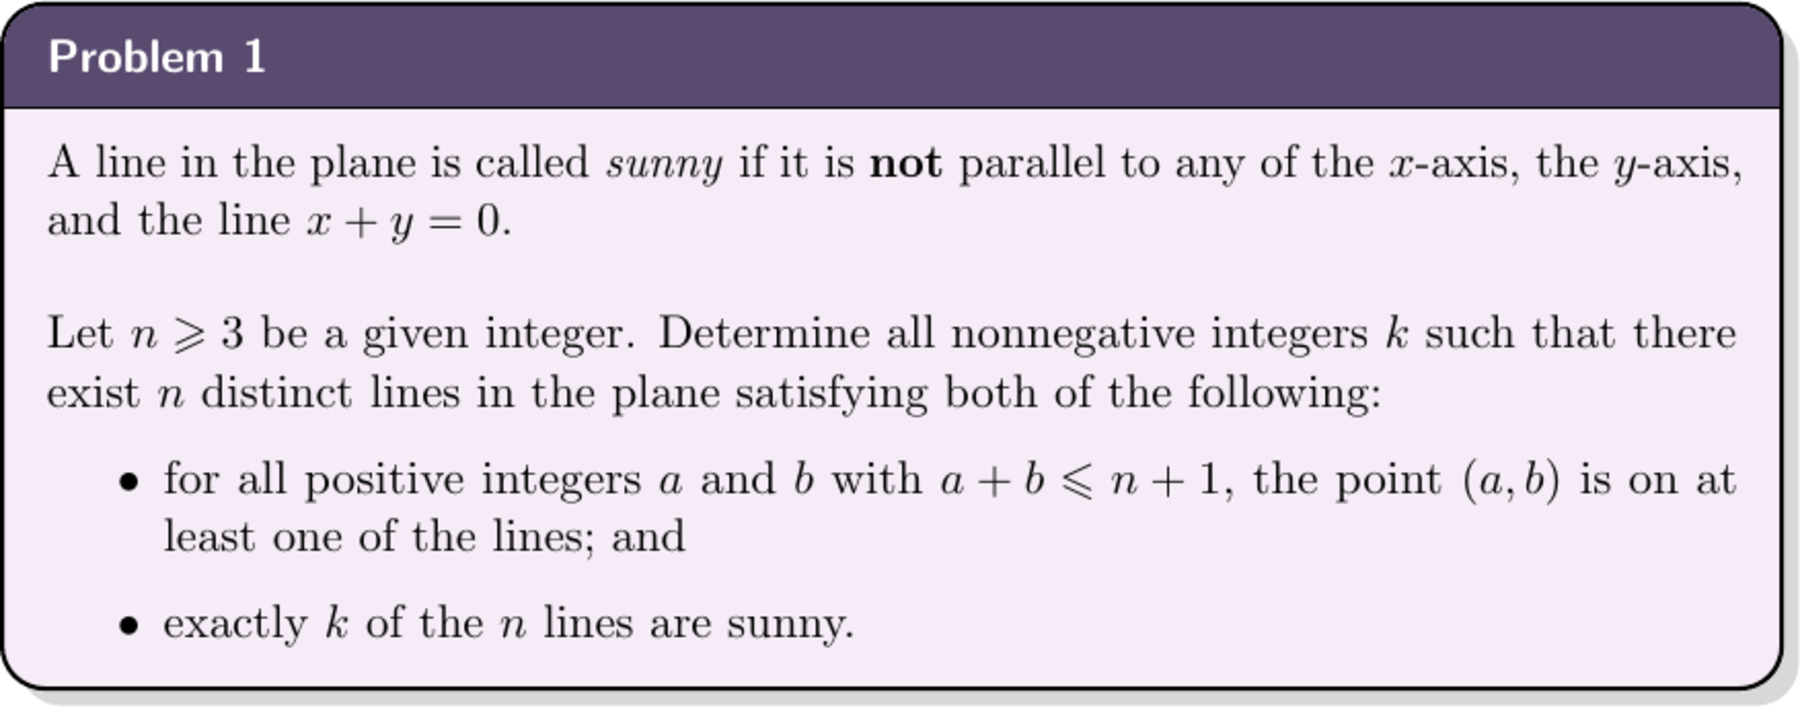
\includegraphics[width=0.98\linewidth,height=0.38\textheight,keepaspectratio]{assets/generated/imo_2025_problem1_crop.png}
\end{examplebox}
\vspace{-0.5mm}
\source{DeepMind 25/07/2024 and 21/07/2025; official IMO 2025 PDF (Deep Think).}
\end{frame}

\planslide{2}

\begin{frame}{Research level: First Proof, from pilot to benchmark}
\footnotesize
\begin{problembox}
\labelline{\problemlabel{}}{reproducible measurement of research-level proving.}
\vspace{-0.3mm}
\scriptsize \keyline{Task}{unseen problems, available human solutions, full write-up; \textbf{criterion}: anonymized acceptance.}
\end{problembox}

\vspace{0.8mm}
\begin{resultbox}
\resultlabel{} : First Batch \(\rightarrow\) Second Batch
\vspace{0.1mm}

\begin{columns}[T,totalwidth=\linewidth]
\column{0.48\linewidth}
\scriptsize
\textbf{\textcolor{aiTeal}{First Batch (02/2026)}}\\[-0.3mm]
\keyline{Signal}{\(\sim\)\textbf{2} clear successes (Q9,Q10).}
\vspace{-0.7mm}
\keyline{Gray zone}{Q5/Q8 close or repairable; no formal review.}

\column{0.50\linewidth}
\scriptsize
\textbf{\textcolor{aiTeal}{Second Batch (03--06/2026)}}\\[-0.3mm]
\keyline{OK}{\textbf{17/39} submissions passed.}
\vspace{-0.7mm}
\keyline{Coverage}{\textbf{7/10} problems had \(\geq 1\) OK solution.}
\vspace{-0.7mm}
\keyline{Criterion}{flawless or minor revisions after anonymized expert review.}
\end{columns}
\end{resultbox}

\vspace{0.8mm}
\begin{takeawaybox}
\scriptsize
\takeawaylabel{} : scale shift, but human validation remains central.
\begin{itemize}
\itemsep0mm
  \keyitem{Capability}{serious proofs possible on nontrivial problems.}
  \keyitem{Costs}{batch 2, \$117--\$4.8k for 10 answers; \(\sim\)\$10--\$480/answer.}
  \keyitem{Bottleneck}{expert review, skipped lemmas, ``standard arguments'', fragile citations.}
  \keyitem{Benchmark}{prompts, logs, tokens, time, costs and acceptance criteria.}
\end{itemize}
\end{takeawaybox}

\vspace{0.2mm}
{\tiny\color{aiSlate}Source: ressources/first-proof-summary.md ; \href{https://1stproof.org/}{1stProof} ; arXiv:2602.05192 ; arXiv:2606.18119.}
\end{frame}

\begin{frame}{Research level: unit distance conjecture}
\begin{columns}[T]
\column{0.47\textwidth}
\scriptsize
\begin{problembox}
\labelline{\problemlabel{}}{\(u(n)\), maximum number of unit-distance pairs among \(n\) points in the plane.}
\end{problembox}

\vspace{-0.2mm}
\begin{examplebox}
{\scriptsize\textbf{OpenAI prompt (summary)}}\\[-0.5mm]
\tiny
\textit{``Resolve Erd\H{o}s's planar unit-distance problem completely.''}\\[-0.2mm]
Prove either \(u(n)\le n^{1+O(1/\log\log n)}\), or counterexamples to every bound
\(n^{1+C/\log\log n}\). \textbf{No partial progress.}
\end{examplebox}

\vspace{-0.2mm}
\begin{resultbox}
\labelline{\resultlabel{}}{OpenAI counterexample, then human verification and optimization.}
\vspace{-0.8mm}
{\centering\scriptsize \(1+o(1)\quad\leadsto\quad\mathbf{1.0152}\)\par}
\vspace{-0.8mm}
{\centering\tiny
\setlength{\tabcolsep}{3pt}
\renewcommand{\arraystretch}{0.84}
\begin{tabular}{@{}lcccc@{}}
\toprule
& Class. & OpenAI & Sawin & Emmerich \\
\midrule
\rowcolor{softTeal}
Exp. & \(1+o(1)\) & \(>1\) & \(1.014\) & \(\mathbf{1.0152}\) \\
\bottomrule
\end{tabular}
\par
}
\end{resultbox}

\vspace{-0.2mm}
\begin{takeawaybox}
\tiny
\labelline{\takeawaylabel{}}{LLM + harness \(\Rightarrow\) PhD-student level on an open problem.}
\end{takeawaybox}

\column{0.52\textwidth}
\centering

\includegraphics[width=\linewidth,height=0.70\textheight,keepaspectratio]{assets/generated/unit_distance_series.pdf}

\vspace{-1mm}
{\tiny\color{aiSlate}\raggedright Sources: OpenAI proof PDF p.3; Alon et al. 2605.20695; Sawin 2605.20579; Emmerich 2606.03419.\par}
\end{columns}
\end{frame}

\begin{frame}{Unit distance: four constructions}
\centering
\vspace{-1mm}
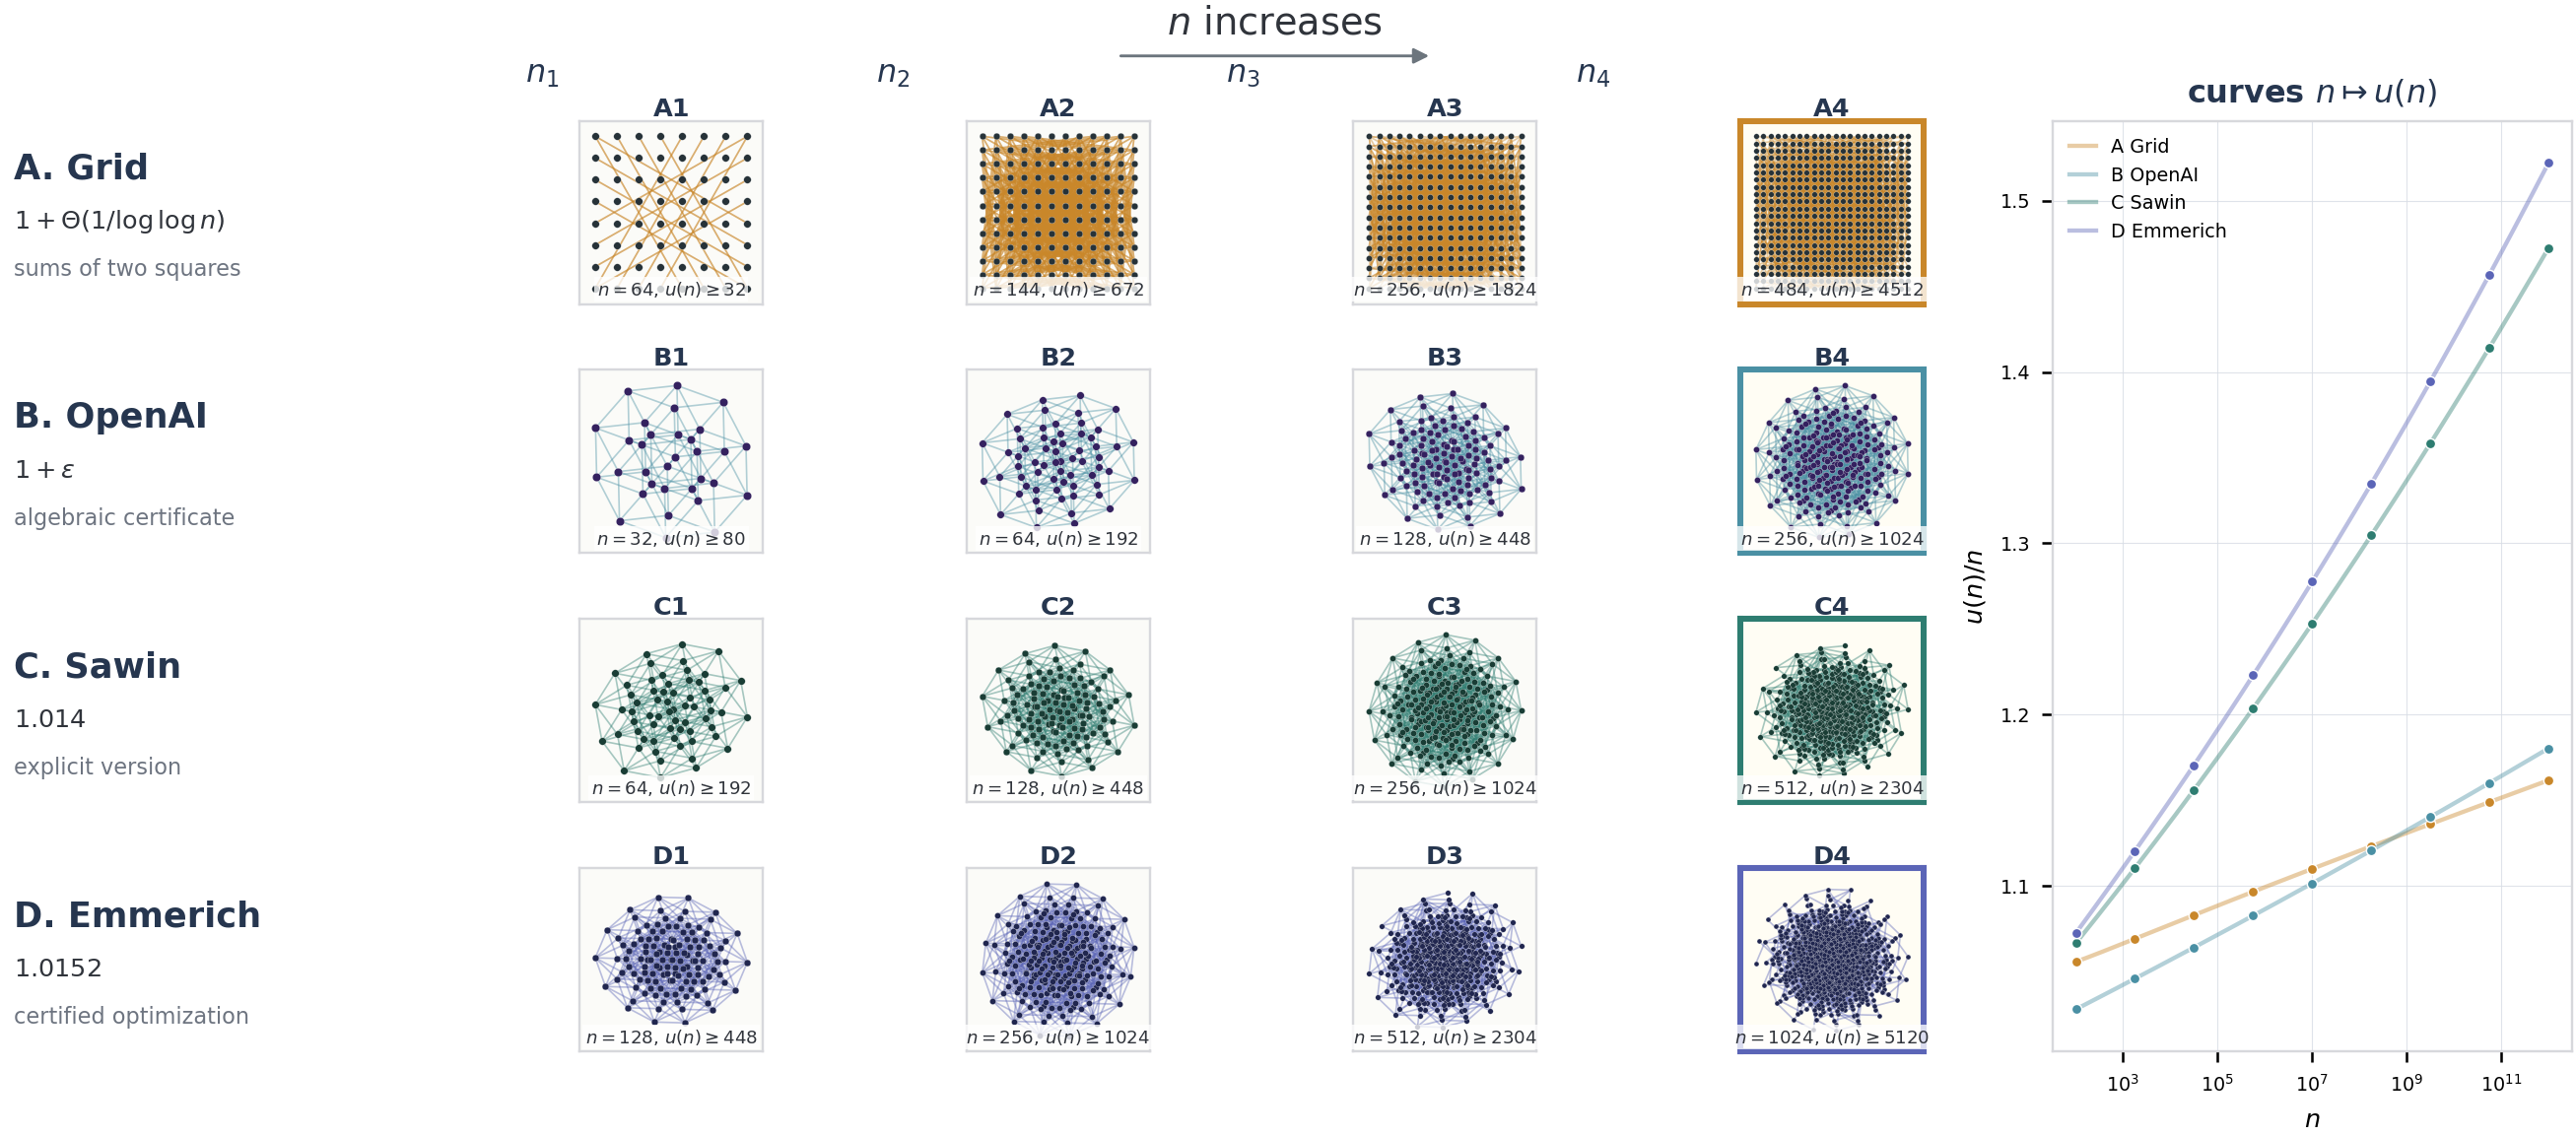
\includegraphics[width=\linewidth,height=0.77\textheight,keepaspectratio]{assets/generated/unit_distance_progress.png}
\vspace{-0.4mm}
{\tiny\color{aiSlate}Sources: Erd\H{o}s 1946; OpenAI proof PDF; Alon et al. 2605.20695; Sawin 2605.20579; Emmerich 2606.03419.\par}
\end{frame}

\begin{frame}{Formal mathematics: Viazovska theorem (Lean)}
\footnotesize
\begin{problembox}
\problemlabel{} : formalize an existing major theorem.
\begin{itemize}
\itemsep0mm
  \keyitem{Object}{optimal packing in dimension \(8\) (Viazovska), extension to dimension \(24\).}
  \keyitem{Stakes}{transfer a very high-level proof into Lean.}
\end{itemize}
\end{problembox}

\vspace{0.6mm}
\begin{resultbox}
\resultlabel{} : public Math, Inc. repository \texttt{Sphere-Packing-Lean}.
\begin{itemize}
\itemsep0mm
  \keyitem{Status}{public, massive Lean project around certification of the \(E_8\) / Leech packing proof.}
  \keyitem{Scope}{geometry of numbers, coding theory, 2022 Fields Medal.}
  \keyitem{Current size}{\textbf{830 files}, \textbf{180\,661 Lean lines}; FLT Lean reference: \textbf{117 files}, \textbf{15\,411 lines}.}
\end{itemize}
\end{resultbox}

\vspace{0.6mm}
\begin{takeawaybox}
\scriptsize
\takeawaylabel{} : large-scale formal certification, but sensitive governance.
\begin{itemize}
\itemsep0mm
  \keyitem{Governance point}{academic (EPFL) \(\rightarrow\) private (Math, Inc.) transfer was highly controversial.}
  \keyitem{Tension}{scientific credit, code maintenance, open Lean infrastructure.}
\end{itemize}
\end{takeawaybox}
\source{GitHub repositories; Hariharan et al., arXiv:2604.23468; local count 09/03/2026 with \texttt{rg} + \texttt{wc -l}.}
\end{frame}

\begin{frame}{Formal mathematics: analysis / PDEs (Lean)}
\footnotesize
\begin{problembox}
\labelline{\problemlabel{}}{formalize modern analysis, still only sparsely covered by \texttt{mathlib}.}
\vspace{-0.3mm}
\scriptsize Standard use case: math expert who is not a Lean specialist, guided by LLM + formal checking.
\end{problembox}

\vspace{0.8mm}
\begin{columns}[T,totalwidth=\linewidth]
\column{0.58\linewidth}
\begin{resultbox}
\labelline{\resultlabel{}}{\textbf{Scott Armstrong} (PDEs) and Julia Kempe; Harnack, Hölder and reusable analysis foundations in \texttt{scottnarmstrong/DeGiorgi}.}
\vspace{-0.4mm}
{\scriptsize\textbf{Short excerpt : \texttt{Harnack.lean}}}\\[-0.7mm]
\begin{beamercolorbox}[wd=\linewidth,rounded=true,sep=0.6mm]{box neutral}
\tiny\ttfamily
\textcolor{aiTeal}{theorem} harnack\\
\quad (A : NormalizedEllipticCoeff d (ball 0 1))\\
\quad (hsol : IsSolution A.1 u) :\\
\quad essSup u \(\mu_{1/2}\) \(\le\)
 exp(C\_harnack d * A.1.\(\Lambda^{1/2}\)) * essInf u \(\mu_{1/2}\) := by ...
\end{beamercolorbox}

\vspace{0.6mm}
\centering

\begin{tikzpicture}[x=1cm,y=1cm]
  \node[draw=aiTeal,fill=softTeal,rounded corners=1pt,inner sep=2pt] (s) at (0,0) {\tiny Sobolev};
  \node[draw=aiTeal,fill=softTeal,rounded corners=1pt,inner sep=2pt] (w) at (1.45,0) {\tiny Weak Harnack};
  \node[draw=aiTeal,fill=softTeal,rounded corners=1pt,inner sep=2pt] (h) at (3.25,0) {\tiny Harnack};
  \node[draw=aiTeal,fill=softTeal,rounded corners=1pt,inner sep=2pt] (r) at (4.55,0) {\tiny Hölder};
  \draw[->,aiTeal] (s) -- (w);
  \draw[->,aiTeal] (w) -- (h);
  \draw[->,aiTeal] (h) -- (r);
\end{tikzpicture}
\end{resultbox}

\column{0.40\linewidth}
\begin{takeawaybox}
\takeawaylabel{}\\[-0.5mm]
\tiny
\begin{itemize}
\itemsep0mm
  \keyitem{Feasibility}{modern analysis with Claude/Codex pro accounts.}
  \keyitem{Expertise}{math guidance essential; impossible outside the domain.}
  \keyitem{Cost}{many tokens, manageable with a solid blueprint.}
  \keyitem{Tension}{math expert vs Lean idiom / core developers.}
  \keyitem{Goal}{formalized foundations to put Lean in the loop.}
\end{itemize}
\end{takeawaybox}
\end{columns}
\vspace{0mm}
{\tiny\color{aiSlate}Source: Armstrong--Kempe, arXiv:2604.05984; \texttt{scottnarmstrong/DeGiorgi}, especially \texttt{Harnack.lean}; Armstrong blog post 07/04/2026.}
\end{frame}

\planslide{3}

\begin{frame}{My research experience}
\begin{columns}[T]
\column{0.58\textwidth}
\scriptsize
\begin{problembox}
\labelline{\problemlabel{}}{make progress on a fairly well-scoped problem where one is stuck; use Lean as a non-specialist.}
\end{problembox}

\vspace{0.5mm}
\begin{resultbox}
\resultlabel{} : personal report from intensive use.
\begin{itemize}
\itemsep0mm
  \keyitem{Unlock}{open problem solved in \textbf{2 weeks} through intensive GPT-5 prompting.}
  \keyitem{Preprint}{\url{https://arxiv.org/abs/2602.01372}}
  \keyitem{Agents}{Codex / Claude Code in daily use.}
  \keyitem{Library}{\url{https://github.com/gpeyre/flow-sinkhorn}}
\end{itemize}
\end{resultbox}

\vspace{0.5mm}
\begin{takeawaybox}
\tiny
\takeawaylabel{} : two regimes and workflow gains.
\begin{itemize}
\itemsep0mm
  \keyitem{Informal}{unlocks open problems.}
  \keyitem{Formal (Lean)}{works, but costs \(\sim 10\times\) more tokens.}
  \keyitem{Writing}{faster prototyping.}
  \keyitem{Technical}{automated repetitive tasks.}
  \keyitem{Reasoning}{Lean certifies the proof without directly improving the mathematical idea.}
\end{itemize}
\end{takeawaybox}
\column{0.42\textwidth}
\centering
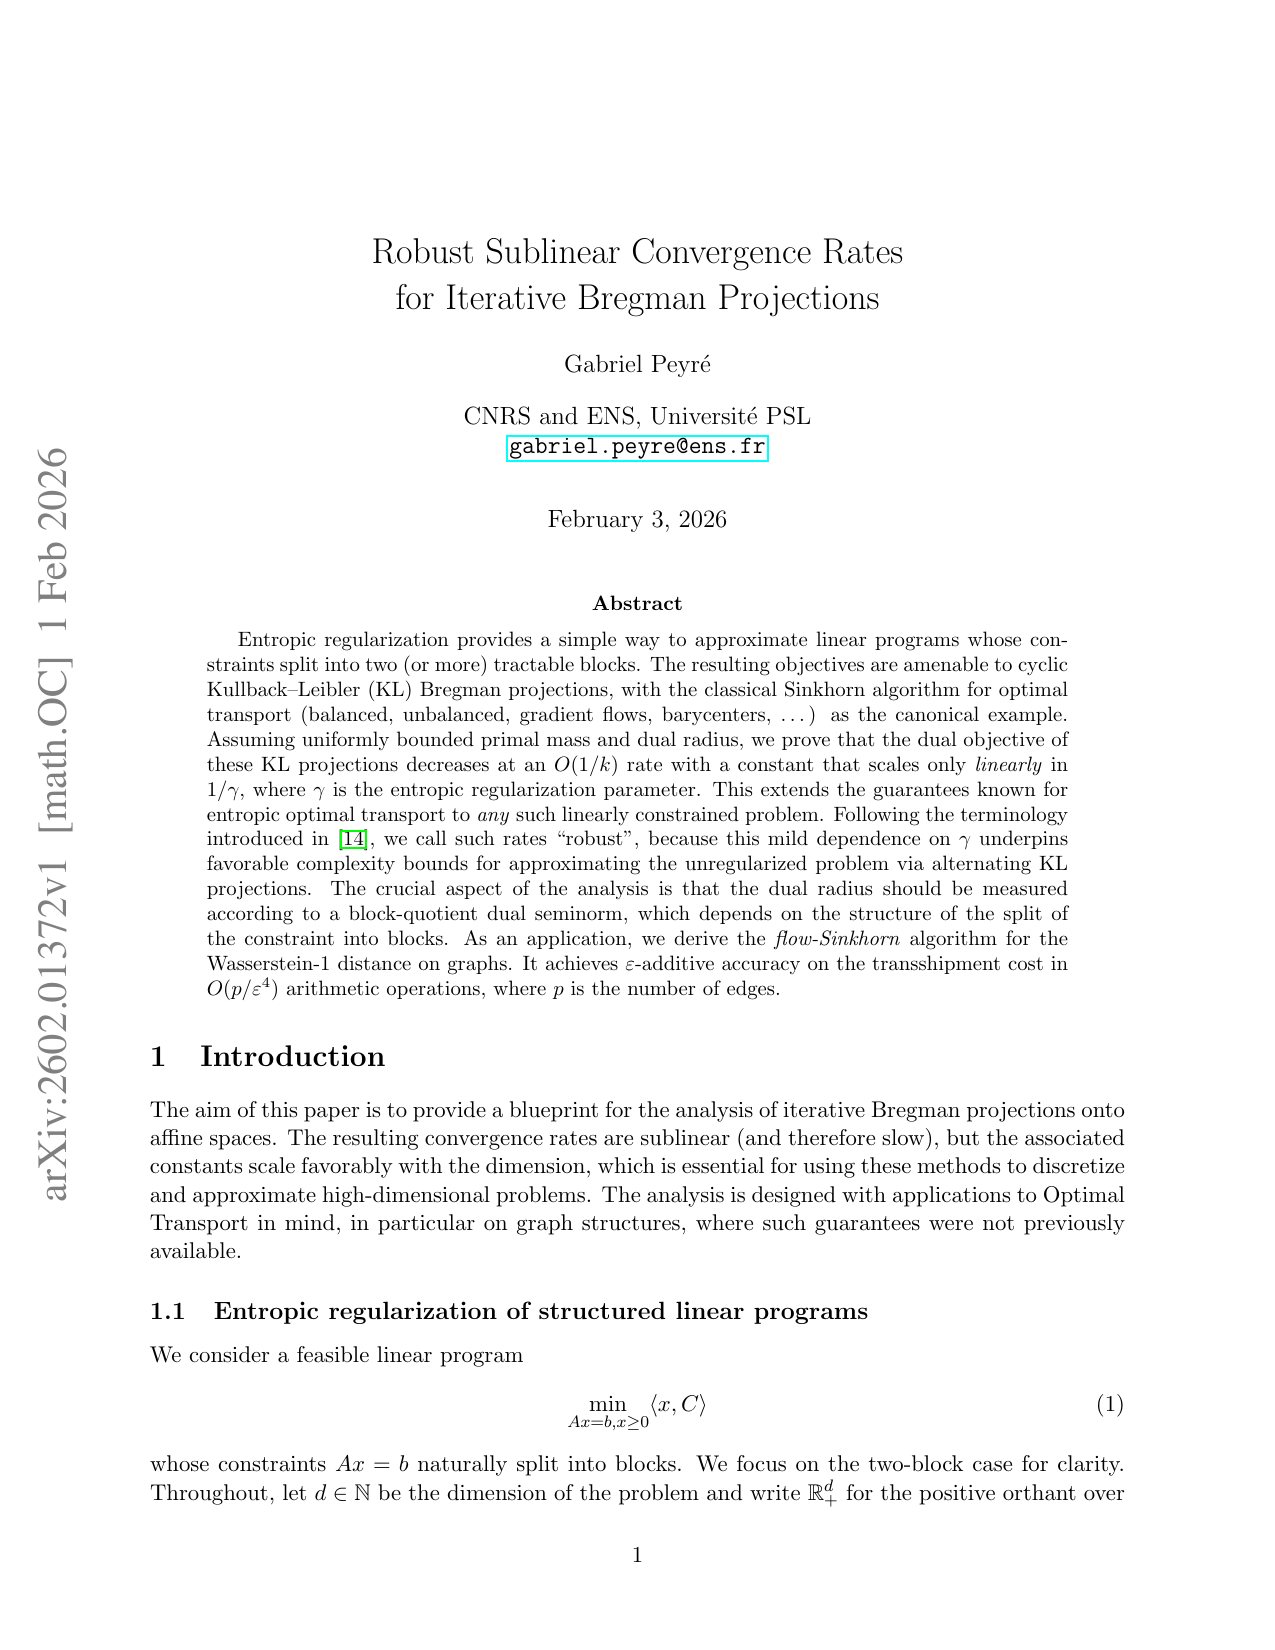
\includegraphics[width=\linewidth,height=0.68\textheight,keepaspectratio]{assets/arxiv_2602_01372_p1.png}
\end{columns}
\source{Personal experience + arXiv/GitHub (accessed 09/03/2026).}
\end{frame}

\begin{frame}{Group experience report}
\begin{columns}[T]
\column{0.55\textwidth}
\scriptsize
\begin{problembox}
\problemlabel{} : collective evaluation at CSD (ENS).
\begin{itemize}
  \keyitem{Protocol}{same prompt, multiple answers.}
  \keyitem{Task}{semi-open question, notebook, code, paper, formalization.}
  \keyitem{Audit}{submissions evaluated across several criteria.}
\end{itemize}
\end{problembox}

\vspace{0.5mm}
\begin{examplebox}
\textbf{Prompt excerpt}\\[-0.3mm]
\tiny\ttfamily
Consider flow matching with a stochastic interpolant a(t)*X0+b(t)*X1.\\
In python/ do an indepth numerical simulation ... X0 sim N(0,Id),\\
X1 is a mixture of three Dirac. In paper/ write a detailed LaTeX article ...\\
compute in closed form Sigma\_t and the flow map T\_t.
\end{examplebox}

\column{0.44\textwidth}
\centering
\fbox{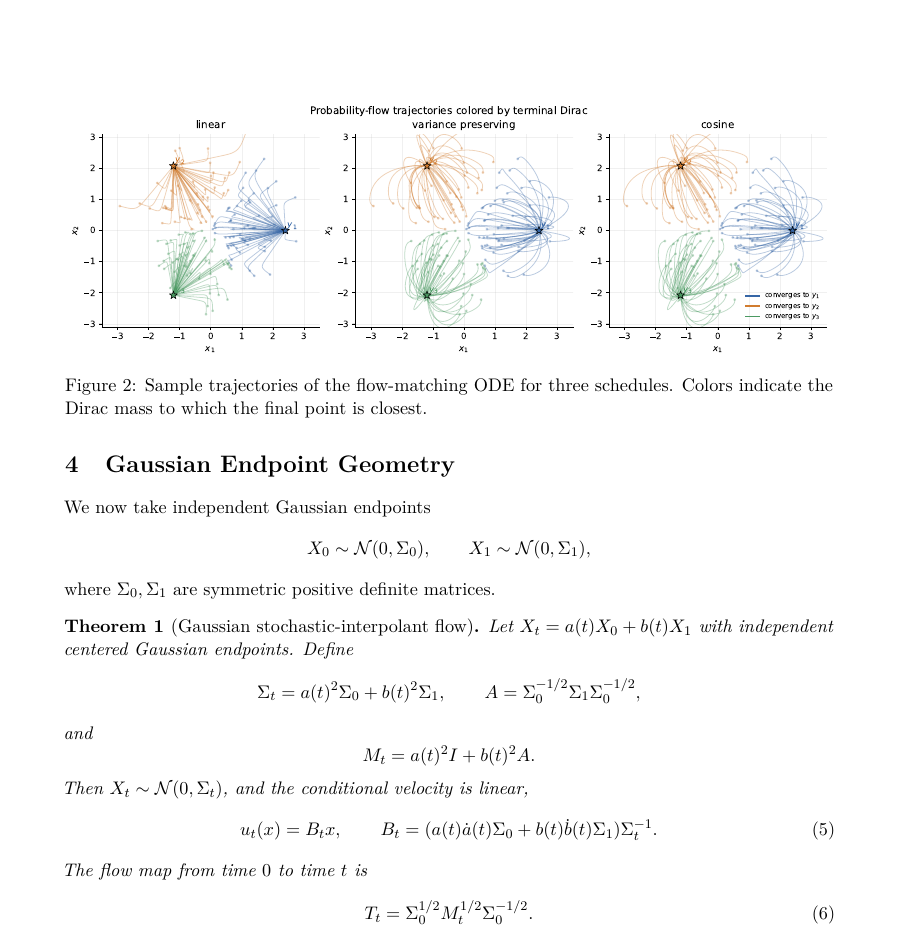
\includegraphics[width=0.90\linewidth,height=0.62\textheight,keepaspectratio]{assets/generated/codex_gabriel_page4_crop.png}}

\vspace{1mm}
\tiny
Snapshot: paper page from the \texttt{codex-gabriel/} submission.
\end{columns}
\source{ressources/agentic-benchs/todo.md; comparative report from 18/06/2026; codex-gabriel submission.}
\end{frame}

\begin{frame}{Group experience report (continued)}
\scriptsize
\begin{problembox}
\problemlabel{} : multicriteria evaluation.
\end{problembox}

\vspace{0.6mm}
\begin{columns}[T,onlytextwidth]
\column{0.53\textwidth}
\scriptsize
\begin{resultbox}
\resultlabel{} : LLM-as-judge aggregation
\vspace{0.3mm}

\centering
\begingroup
\tiny
\setlength{\tabcolsep}{3pt}
\renewcommand{\arraystretch}{0.78}
\begin{tabular}{@{}lccc@{}}
\toprule
Submission & Math & Code & Overall \\
\midrule
\rowcolor{softTeal}
emmanuel & 9.3 & 8.8 & 9.1 \\
\rowcolor{softTeal}
codex-gabriel & 9.0 & 9.0 & 8.8 \\
openclaw & 8.2 & 8.6 & 8.2 \\
hermes & 7.8 & 8.0 & 7.7 \\
claude-gabriel & 6.5 & 7.5 & 7.1 \\
codex-kimia & 7.0 & 7.0 & 7.0 \\
codex-clement & 7.0 & 5.5 & 6.2 \\
antigravity-a. & 5.8 & 6.0 & 5.8 \\
antigravity-o. & 5.5 & 5.0 & 5.4 \\
\bottomrule
\end{tabular}
\endgroup

\vspace{0.2mm}
\raggedright
\tiny Overall = aggregation of math, code, paper and robustness criteria.
\end{resultbox}

\column{0.45\textwidth}
\scriptsize
\begin{resultbox}
\resultlabel{} : robust signals
\begin{itemize}
\itemsep0mm
  \keyitem{Math}{Codex \(\gg\) Claude \(\gg\) rest.}
  \keyitem{Code}{Claude \(\gg\) Codex \(\gg\) rest.}
  \keyitem{Budget}{performance \(\simeq\) tokens.}
\end{itemize}
\end{resultbox}

\vspace{0.1mm}
\begin{takeawaybox}
\takeawaylabel{} : effect of token budget
\vspace{0mm}

\tiny
\renewcommand{\arraystretch}{0.82}
\begin{tabular}{@{}p{0.28\linewidth}p{0.64\linewidth}@{}}
\toprule
Budget & Typical outcome \\
\midrule
\rowcolor{softRed}
Small & incorrect proof \\
\rowcolor{softAmber}
Medium & proof OK, statement imperfect \\
\rowcolor{softTeal}
Large & complete solution \\
\rowcolor{softGreen}
Huge & Lean viable \\
\bottomrule
\end{tabular}
\end{takeawaybox}
\end{columns}
\vspace{-2.0mm}
{\tiny\color{aiSlate}Source: CSD experiment; audit ressources/agentic-benchs/report.\par}
\end{frame}

\begin{frame}{Zoom: Emmanuel Sérié / Noogram}
\scriptsize
\begin{columns}[T,totalwidth=\linewidth]
\column{0.45\linewidth}
\begin{problembox}
\problemlabel{} : CSD prompt \(\rightarrow\) full scientific artifact.
\end{problembox}

\vspace{0.6mm}
\begin{resultbox}
\resultlabel{} : Noogram contribution
\begin{itemize}
\itemsep0mm
  \keyitem{Theorem}{Gaussian FM \(=\) OT iff covariances commute.}
  \keyitem{Artifacts}{site, code, paper, figures, Lean, report.}
  \keyitem{Audit}{false proof found and fixed; score \(\mathbf{9.1}\).}
\end{itemize}
\end{resultbox}

\vspace{0.6mm}
\begin{takeawaybox}
\takeawaylabel{} : agent harnessing for science.
\begin{itemize}
\itemsep0mm
  \keyitem{Chain}{generate, test, refute, publish.}
  \keyitem{Rigor}{Lean as anchor; expert required.}
  \keyitem{Cost}{heavy, but auditable end to end.}
\end{itemize}
\end{takeawaybox}

\column{0.53\linewidth}
\centering
\fbox{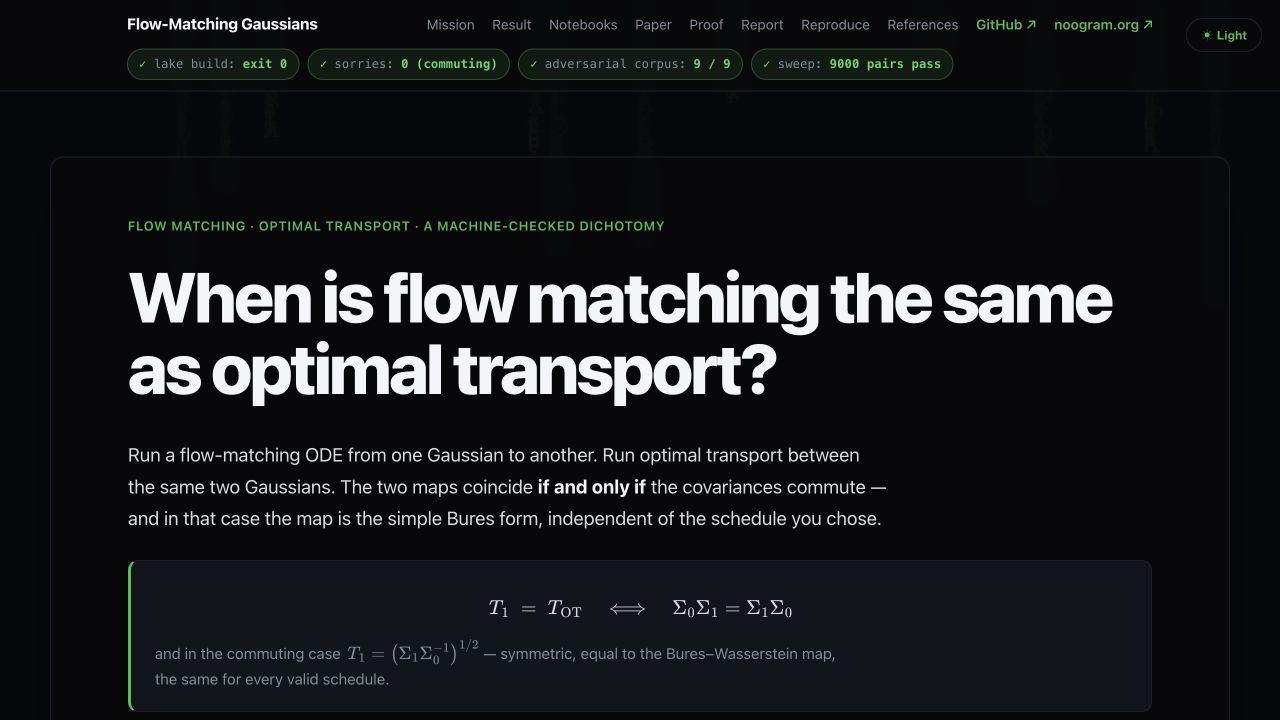
\includegraphics[width=0.98\linewidth,height=0.31\textheight,keepaspectratio]{assets/generated/noogram_flow_matching_site.png}}

\vspace{0.8mm}
\fbox{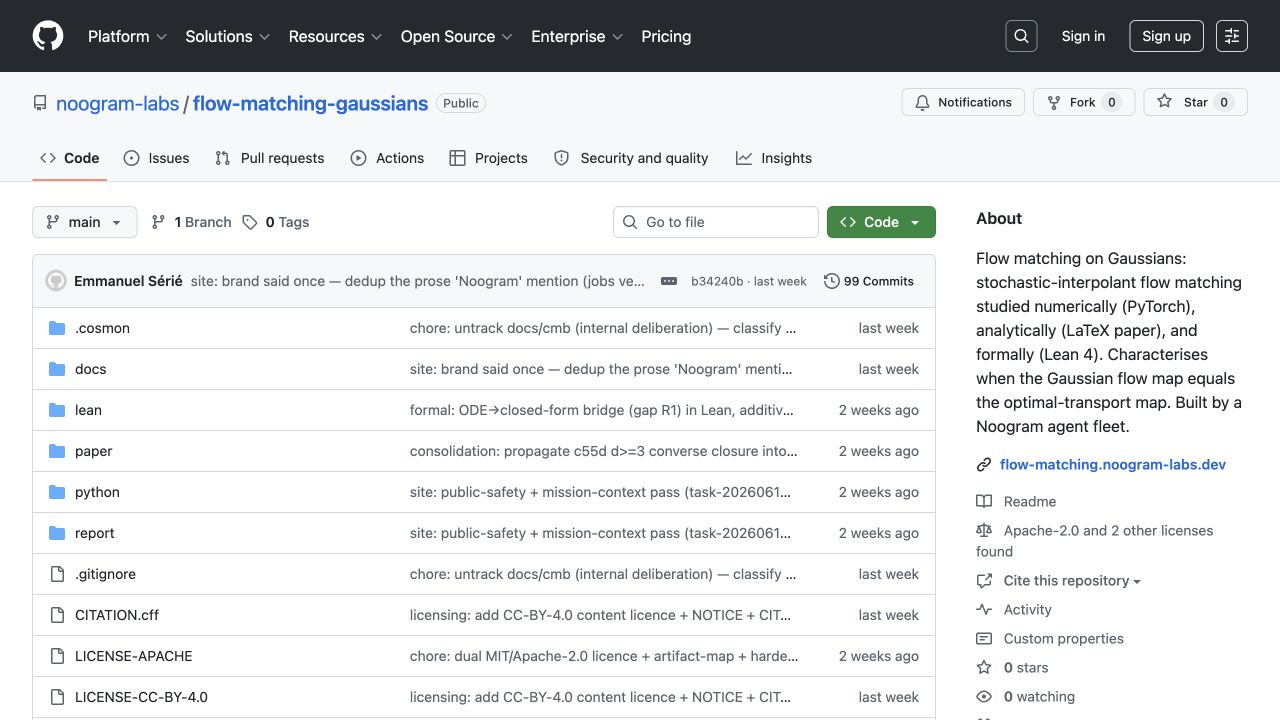
\includegraphics[width=0.98\linewidth,height=0.27\textheight,keepaspectratio]{assets/generated/noogram_flow_matching_github.png}}

\vspace{0.4mm}
{\tiny\color{aiSlate}\raggedright Sources: Noogram site; GitHub \texttt{noogram-labs/flow-matching-gaussians}; CSD audit.\par}
\end{columns}
\end{frame}

\planslide{4}

\begin{frame}{Impact on evaluation and teaching}
\small
\begin{minipage}[t]{0.48\linewidth}
\vspace{0pt}
\begin{neutralboxalt}
\textbf{Reviewing}: AI as first reader
\vspace{0.6mm}

\centering
\fbox{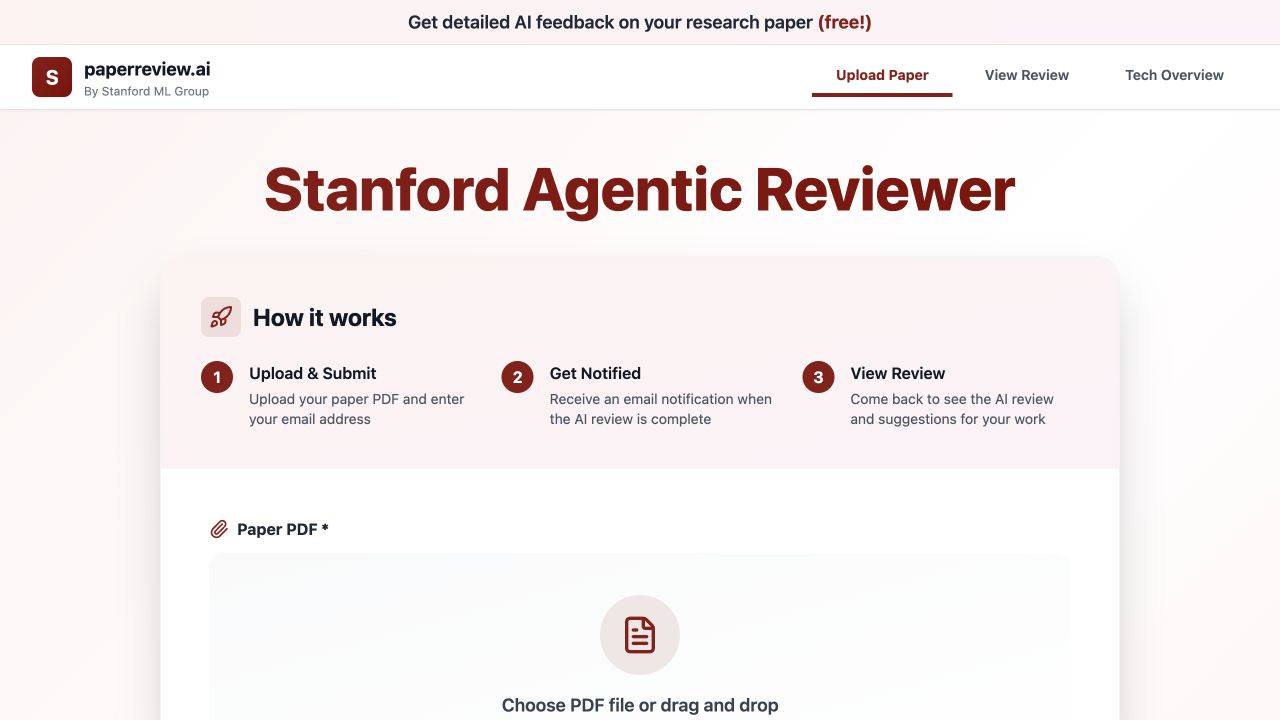
\includegraphics[width=0.93\linewidth,height=0.31\textheight,keepaspectratio]{assets/generated/paperreview_ai_screenshot.png}}

\vspace{0.6mm}
\raggedright
\scriptsize
\begin{itemize}
\itemsep0mm
  \keyitem{Automation}{first report, local flaws, suggestions.}
  \keyitem{Weak signal}{triage, not scientific validation.}
  \keyitem{Human value}{validity, novelty, taste.}
\end{itemize}
\end{neutralboxalt}
\end{minipage}\hfill
\begin{minipage}[t]{0.48\linewidth}
\vspace{0pt}

\begin{neutralbox}
\textbf{Teaching}: preserve human training
\vspace{0.5mm}

\scriptsize
\begin{itemize}
\itemsep0.4mm
  \keyitem{Level}{PhD-level writing, code, local critique.}
  \keyitem{Risk}{delegating before learning to reason.}
  \keyitem{Loss}{future teachers, reviewers, AI evaluators.}
  \keyitem{Protect}{oral exams, proof critique, AI audit.}
\end{itemize}
\end{neutralbox}
\end{minipage}
\source{\href{https://paperreview.ai/}{PaperReview.ai}, Stanford ML Group (screenshot 02/07/2026) ; qualitative synthesis.}
\end{frame}

\begin{frame}{Actions for the community}
\footnotesize
\begin{columns}[T,totalwidth=\linewidth]
\column{0.49\linewidth}
\begin{actionbox}
\begin{columns}[T,totalwidth=\linewidth]
\column{0.62\linewidth}
\textbf{Structure the community}
\column{0.34\linewidth}
\vspace{-1.4mm}
\centering

\includegraphics[width=\linewidth,height=0.10\textheight,keepaspectratio]{assets/generated/aissai_logo.png}
\end{columns}
\vspace{-1.2mm}
\begin{itemize}
\itemsep0mm
  \keyitem{CNRS RT}{bridge AI, math, formalization, CS (INSMI/INS2I).}
  \keyitem{AISSAI}{``AI for mathematics'' quarter with the RT.}
\end{itemize}
\end{actionbox}

\vspace{1.4mm}
\begin{claimbox}
\textbf{Open access to models}
\begin{itemize}
  \keyitem{Repos}{academic projects connected to models.}
  \keyitem{Models}{control and auditability.}
\end{itemize}
\end{claimbox}

\column{0.49\linewidth}
\begin{examplebox}
\textbf{Dialogue with industry}
\begin{itemize}
  \keyitem{DeepMind}{funds AISSAI postdoc program.}
  \keyitem{Mistral}{Emmy tools for CNRS to develop further.}
\end{itemize}
\end{examplebox}

\vspace{1.4mm}
\begin{riskbox}
\textbf{Do not forget training}
\begin{itemize}
  \keyitem{Faculty}{design + evaluation.}
  \keyitem{Evaluators}{preserve human training.}
\end{itemize}
\end{riskbox}
\end{columns}
\end{frame}

\begin{frame}{Conclusion}
\footnotesize
\begin{columns}[T,totalwidth=\linewidth]
\column{0.49\linewidth}
\begin{claimbox}
\textbf{1. Acceleration already visible}
\begin{itemize}
  \keyitem{Performance}{\textbf{very fast} progress.}
  \keyitem{Workflows}{code, verify, write.}
\end{itemize}
\end{claimbox}

\vspace{1.4mm}
\begin{proofbox}
\textbf{2. Concrete scientific impact}
\begin{itemize}
  \keyitem{Informal}{open problems unlocked.}
  \keyitem{Formal}{Lean progressing, high token cost.}
\end{itemize}
\end{proofbox}

\column{0.49\linewidth}
\begin{examplebox}
\textbf{3. Human role displaced}
\begin{itemize}
  \keyitem{Positioning}{augment, not replace.}
  \keyitem{Role}{researcher \(\rightarrow\) judge of proof quality.}
\end{itemize}
\end{examplebox}

\vspace{1.4mm}
\begin{riskbox}
\textbf{4. Collective stakes}
\begin{itemize}
  \keyitem{Access}{controllable and auditable models.}
  \keyitem{Tension}{academic--industry exchanges.}
  \keyitem{Sovereignty}{scientific and institutional framing.}
\end{itemize}
\end{riskbox}
\end{columns}
\end{frame}

\end{document}
